% Editing notes
% - No tabs, just spaces!
% - No hanging whitespace
% - Wrap lines to 79 characters
% - Indentation should be two spaces per indent
% - Only one space after periods.
% - Don't worry about formatting details, just get the content in place.

\documentclass{article}

\usepackage{graphicx}
\usepackage{booktabs} % for table /toprule, /midrule, etc
\usepackage{todo}

\title{Perturbed Gait Data}

\begin{document}

\begin{abstract}

  Herein we share a typical gait data set collected from 11 subjects walking at
  a three speeds on an instrumented treadmill while being longitudinally
  perturbed during each stance phase with pseudo-random fluctuations in the
  speed of the treadmill belt. We provide raw marker and ground reaction loads in addition
  to a presentation of processed data that includes gait landmarks, 2D joint
  angles, angular rates, and joint torques and the software that does the
  processing. The protocol is described in detail along with the additional
  meta data about each of the data files. This data can be useful for
  validating or generating mathematical models that capable of simulating
  non-periodic and perturbed gaits.

\end{abstract}

\section{Introduction}
%
Emerging powered prosthetics are in need of bio-inspired control systems.
Ideally, a powered prosthetic would behave in such a way that the user would
feel like their limb was never disabled. There are a variety of approaches to
developing bio-inspired control systems some of which aim to mimic the
reactions and motion of an able-bodied person. A modern gait lab is able to
collect a variety of kinematic, kinetic, and physiological data from humans
during gait. This data can potentially be used to drive the design of the human
mimicking controller. With a rich enough data set, one may be able to identify
control mechanism used during a human's natural gait and recovery from
perturbations. We have collected data that we believe is richer than previous
gait data sets and may be rich enough for control identification. The data can
also be used for verification purposes for controllers that have been designed
in other manners.

We collected over five and half hours of perturbed gait data from 11 subjects
sampled at 100 hz. The data has been organized and made available for other
research uses.

\section{Equipment}
%
The Human Motion and Control Lab at Cleveland State University has modern human
motion measurement equipment. Our system includes:

\begin{itemize}
  \item A ForceLink R-Mill which has dual 6 degree of freedom force plates,
    independent belts for each foot, and lateral and pitch motion capabilities.
  \item A 10 Camera Motion Analysis motion capture system which includes Osprey
    cameras, the Cortex software, and hardware for collecting analog and camera
    data simultaneously. Delsys wireless EMG + 3D Accelerometers.
  \item Motek Medical’s D-Flow software and visual display system.
\end{itemize}

Cortex alone is capable of delivering data from the cameras along with force
plates, and analog sensors (EMG/Accelerometer) through a National Instruments
XXXX data acquisition unit. D-Flow is required to collect data from any digital
sensors and the treadmill's motion (lateral, pitch, and belts). D-Flow can
output multiple types of files which contain the different data.

Our motion capture system's coordinate system is such that the X coordinate
points to the right, the Y coordinate points upwards, and the Z coordinate
follows from the right-hand-rule, i.e. points backwards with respect to a
person walking forward on the treadmill. The camera's coordinate system is
aligned to an origin point on treadmill's surface during camera calibration.
The same point is used as the origin of the ground reaction force measuring
system.

\section{Raw Data}
%
The raw data consists of a set of ASCII tab delimited text files output from
both the ``mocap'' and ``record'' modules in D-Flow in addition to a YAML file
that contains all of the necessary meta data for the given trial. These three
files are stored in a hierarchy of directories with one trial per directory.
The directories are named in the following fashion \verb+T001/+ where \verb+T+
stands for ``trial'' and the following three digits are provide a unique trial
identification number.

The text file output from the mocap module in DFlow is a tab delimited file.
The first line is the header and contains a time stamp column, frame number
column, marker position columns, force plate force/moment columns, force plate
center of pressure columns, other analog columns, and potentially results from
the real time Human Body Model \cite{Bogert2013} which is included with the
D-Flow software. These are detailed below. The numerical values of the
measurements are provided in decimal floating point notation with 6 decimals of
precision, e.g. 123456.123456 [\%1.6f].

\subsection{mocap-xxx.txt}

The output from the D-Flow mocap module is stored in a tab delimited file named
\verb+mocap-xxx.txt+ where \verb+xxx+ represents the trial id number. The file
contains several columns:

\begin{description}
  \item[TimeStamp] The monotonically increasing computer clock time when D-Flow
    recieves a frame from Cortex. These are approximately at 100 hz and given
    in seconds.
  \item[FrameNumber] Monotonically increasing positive integers that correspond
    to each frame received from Cortex.
  \item[Marker Coordinates] Any column that ends in \verb+.PosX+, \verb+.PosY+,
    or \verb+.PosZ+ are marker coordinates expressed in Cortex's Cartesian
    reference frame. These values are in meters.
  \item[Ground Reaction Loads] There are three ground reaction forces and three
    ground reaction moments recorded by each of the two force plates in Newtons
    and Newton-Meters, respectively. The prefix for these columns is either
    \verb+FP1+ or \verb+FP2+ and represents either force plate 1 (left) or 2
    (right). The suffixes are either \verb+.For[XYZ]+, \verb+.Mom[XYZ]+ for the
    forces and moments, respectively. The force plate voltages are sampled at a
    much higher frequency than the cameras, but delivered at the Cortex camera
    sample rate, 100 Hz through the D-Flow mocap module. A force/moment
    calibration matrix stored in Cortex converts the voltages to forces and
    moments before sending it to D-Flow [1]. Cortex also computes the center of
    pressure from the forces, moments, and force plate dimensions. These have
    the same prefixes for the plate number, have the suffix \verb+.Cop[XYZ]+,
    and are in meters.
  \item[Analog Channels] Several analog signals are recorded under column
    headers \verb+Channel[1-99].Anlg+. These correspond to analog signals
    sampled by Cortex and correspond to the 96 analog-channel National 
    Instruments 6255 DAQ box. The first twelve are the voltages from the 
    force plate load cells. We also record the acceleration of 4 points on the
    treadmill base in channels 61-72.  TvdB: are these useful?  If so, we need to 
    provide information on how to process these channels.  If not, maybe
    not mention them at all?
\end{description}

\subsection{record-xxx.txt}
%
The record module also outputs a tab delimited ASCII text file. It includes a
\verb+Time+ column which records the D-Flow system time in seconds which
corresponds to the time recorded in the \verb+TimeStamp+ column in mocap module
tsv file. There are two additional columns \verb+RightBeltSpeed+ and
\verb+LeftBeltSpeed+ which provide the independent belt speeds measured in
meters per second by an encoder in the treadmill.

Finally, the record module is capable of recording the time at which various
events occur, as detected or set by D-Flow. It does this by inserting commented
(\#) lines in between the rows when the event occurred. The record files have
several events that correspond to the phases of the protocol:

\begin{description}
  \item[A: Force Plate Zeroing] Marks the time at which there is no load on the
    force plates and when the voltages were zeroed.
  \item[B: Calibration Pose] Marks the time at which the person is in the
    T-Pose.
  \item[C: First Normal Walking] Marks the time when the treadmill begins Phase
    1: constant belt speed.
  \item[D: Longitudinal Perturbation] Marks the time when the treadmill begins
    Phase 2: longitudinal perturbations in the belt speed.
  \item[E: Second Normal Walking] Marks the time when phase 3 starts: constant
    belt speed.
  \item[F: Unloaded End] Marks the time at which there is no load on the force
    plates and the belts are stationary.
\end{description}

\subsection{meta-xxx.yml}

Each trial directory contains a meta data file in the YAML format. There are
three main headings: \verb+study+, \verb+subject+, and \verb+trial+.

The \verb+study+ section contains identifying information for the overall
study, an identification number, name, and description. This is the same for
all meta data files in the study.

The \verb+subject+ provides key value pairs of information about the subject in
that trial. Each subject has a unique identification number and basic
anthropomorphic data is included.

The \verb+trial+ section contains the unique information about the trial. Each
trial has a unique identification number.

An example meta data file is shown in Figure \ref{fig:example-meta-data} and
the following gives and explanation of the contents.

\begin{figure}
  \small
  \begin{verbatim}
    study:
            id: 1
            name: Gait Control Identification
            description: Perturb the subject during walking and running.
    subject:
            id: 0
    trial:
            id: 58
            subject-id: 0
            datetime: 2014-03-28
            notes: >
                    This is an unloaded trial (no subject) 10 minute protocol that
                    perturbs the subject longitudinally. The treadmill reference
                    markers were not in place. We have the four custom made metal
                    feet placed under the four corners of the treadmill to prevent
                    pitch and sway movements. In addition, we also have the front
                    left and rear right feet that were installed by Motek. We also
                    have +/-3g analog accelerometers (ADXL330) affixed to the four
                    corners of the main frame of the treadmill and wired into the
                    NI box. The right handrail is removed.
            nominal-speed: 0.8
            nominal-speed-units: meters per second
            stationary-platform: True
            pitch: False
            sway: False
            hardware-settings:
                    high-performance: True
            analog-channel-map:
                    Channel1.Anlg: F1Y1
                    Channel2.Anlg: F1Y2
                    Channel3.Anlg: F1Y3
                    Channel4.Anlg: F1X1
                    Channel5.Anlg: F1X2
                    Channel6.Anlg: F1Z1
                    Channel7.Anlg: F2Y1
                    Channel8.Anlg: F2Y2
                    Channel9.Anlg: F2Y3
                    Channel10.Anlg: F2X1
                    Channel11.Anlg: F2X2
                    Channel12.Anlg: F2Z1
                    Channel61.Anlg: Front_Left_AccX
                    Channel62.Anlg: Front_Left_AccY
                    Channel63.Anlg: Front_Left_AccZ
                    Channel64.Anlg: Back_Left_AccX
                    Channel65.Anlg: Back_Left_AccY
                    Channel66.Anlg: Back_Left_AccZ
                    Channel67.Anlg: Front_Right_AccX
                    Channel68.Anlg: Front_Right_AccY
                    Channel69.Anlg: Front_Right_AccZ
                    Channel70.Anlg: Back_Right_AccX
                    Channel71.Anlg: Back_Right_AccY
                    Channel72.Anlg: Back_Right_AccZ
            events:
                    A: Force Plate Zeroing
                    B: Calibration Pose
                    C: First Normal Walking
                    D: Longitudinal Perturbation
                    E: Second Normal Walking
                    F: Unloaded End
            files:
                    mocap: mocap-058.txt
                    record: record-058.txt
                    meta: meta-058.yml
  \end{verbatim}
  \caption{An example meta data YAML file.}
  \label{fig:example-meta-data}
\end{figure}

\begin{description}
  \item[analog-channel-map] A key value mapping of strings specifying the name
    of the signal emmitted from the analog channels of the NI USB XXX.
  \item[cortex-version] (string) Matches the version of Cortex used to record
    the trial.
  \item[datetime] (string) A date formatted string giving the date and/or time
    of the trial in the \verb|YYYY-MM-DD| format.
  \item[dflow-version] (string) Matches the version of D-Flow used to record
    the trial.
  \item[events] A key value map which prescribes names to the events recorded
    in the record file.
  \item[files] (list) A key value mapping of files associated with this trial
    where the key is the file type and the values are the path to the file
    relative to this meta file.
  \item[hardware-settings] There are tons of settings for the hardware in both
    D-Flow, Cortex, and the other software in the system. This contains any
    non-default settings.
    \begin{description}
      \item[high-performance] (boolean) Indicates whether the D-Flow high
        performance setting was on (True) or off (False).
    \end{description}
  \item[id] (integer) A unique three digit identifier for the trial. All of the
    file names and directories associated with this trial include this.
  \item[marker-map] A string key value map which contains names for the
    markers.
  \item[marker-set] (string) Indicates the HBM \cite{Bogert2013} marker
    set used during the trial, either full, lower, or NA.
  \item[nominal-speed] (float) The nominal or base speed during the trial.
  \item[nominal-speed-units] (string) The units of the nominal speed.
  \item[notes] {string} Notes about the trial.
  \item[pitch] (boolean) Indicates if the pitch degree of freedom was acutated
    during the trial.
  \item[stationary-platform] (boolean) Indicates whether the treadmill
      sway or pitch motion was actuated during the trial. If this flag is
      false, the measured ground reaction forces must be compensated for the
      inertial affects and be expressed the forces and moments in the motion
      capture reference frame.
  \item[subject-id] (integer) A number corresponding to the subject in the
    trial.
  \item[sway] (boolean) Indicates if the lateral (sway) degree of freedom was
    acutated during the trial.
\end{description}

\subsection{Markers}
%
We make use of the full body 47 marker set described in \cite{Ton's HBM paper}
and presented in detail in Table \ref{tab:marker-labels}. As with all camera
based motion capture systems, the markers sometimes go missing in the
recording.

If the data was recorded in a D-Flow version less than 3.16.2rc4 [3], D-Flow
records the last non-missing value in all three axes until the marker is
visible again when a marker goes missing.

In D-Flow versions greater than or equal to 3.16.2rc4 the missing markers are
indicated in the TSV file as either 0.000000 or -0.000000, which is the same as
has been in the HBM columns in all versions of D-Flow. The D-Flow version must
be provided in the meta data yml file, otherwise it will assume D-Flow is at
the latest version.

\begin{table}
  \caption{Descriptions of the 47 markers used in this study.}
  \centering
  \small
  \begin{tabular}{rlll}
    \toprule
    Number & Label & Name & Description \\
    \midrule
    1  & LHEAD & Left head                             & Just above the ear, in the middle. \\
    2  & THEAD & Top head                              & On top of the head, in line with the LHEAD and RHEAD. \\
    3  & RHEAD & Right head                            & Just above the ear, in the middle. \\
    4  & FHEAD & Forehead                              & Between line LHEAD/RHEAD and THEAD a bit right from center. \\
    5  & C7    & C7                                    & On the 7th cervical vertebrae. \\
    6  & T10   & T10                                   & On the 10th thoracic vertbrae. \\
    7  & SACR  & Sacrum bone                           & on the scacral bone. \\
    8  & NAVE  & Navel                                 & On the navel. \\
    9  & XYPH  & Xiphoid process                       & Xiphoid process of the sternum. \\
    10 & STRN  & Sternum                               & On the jugular notch of the sternum. \\
    11 & BBAC  & Scapula                               & On the inferior angle fo the right scapular. \\
    12 & LSHO  & Left shoulder                         & Left acromion. \\
    13 & LDELT & Left deltoid muscle                   & Apex of the deltoid muscle. \\
    14 & LLEE  & Left lateral elbow                    & Left lateral epicondyle of the elbow. Upper one in the T-Pose. \\
    15 & LMEE  & Left medial elbow                     & Left medial epicondyle of the elbow. Lower on in the T-Pose. \\
    16 & LFRM  & Left forearm                          & On 2/3 on the line between the LLEE and LMW. \\
    17 & LMW   & Left medial wrist                     & On styloid process radius, thumb side. \\
    18 & LLW   & Left lateral wrist                    & On styloid process ulna, pinky side. \\
    19 & LFIN  & Left fingers                          & Center of the hand. Caput metatarsal 3. \\
    20 & RSHO  & Right shoulder                        & Right acromion. \\
    21 & RDELT & Right deltoid muscle                  & Apex of deltoid muscle. \\
    22 & RLEE  & Right lateral elbow                   & Right lateral epicondyle of the elbow. Lower one in the T-pose. \\
    23 & RMEE  & Right medial elbow                    & Right medial epicondyle of the elbow. Lower one in the T-pose. \\
    24 & RFRM  & Right forearm                         & On 1/3 on the line between the RLEE and RMW. \\
    25 & RMW   & Right medial wrist                    & On styloid process radius, thumb side. \\
    26 & RLW   & Right lateral wrist                   & On styloid process ulna, pinky side. \\
    27 & RFIN  & Right fingers                         & Center of the hand. Caput metatarsal 3. \\
    28 & LASIS & Pelvic bone left front                & Left anterior superior iliac spine. \\
    29 & RASIS & Pelvic bone right front               & Right anterior superior iliac spine. \\
    30 & LPSIS & Pelvic bone left back                 & Left posterior superio iliac spine. \\
    31 & RPSIS & Pelvic bone right back                & Right posterior superior iliac spine. \\
    32 & LGTRO & Left greater trochanter of the femur  & On the cetner of the left greater trochanter. \\
    33 & FLTHI & Left thigh                            & On 1/3 on the line between the LFTRO and LLEK. \\
    34 & LLEK  & Left lateral epicondyle of the knee   & On the lateral side of the joint axis. \\
    35 & LATI  & Left anterior of the tibia            & On 2/3 on the line between the LLEK and LLM. \\
    36 & LLM   & Left lateral malleoulus of the ankle  & The center of the heel at the same height as the toe. \\
    37 & LHEE  & Left heel                             & Center of the heel at the same height as the toe. \\
    38 & LTOE  & Left toe                              & Tip of big toe. \\
    39 & LMT5  & Left 5th metatarsal                   & Caput of the 5th metatarsal bone, on joint line midfoot/toes. \\
    40 & RGTRO & Right greater trochanter of the femur & On the cetner of the right greater trochanter. \\
    41 & FRTHI & Right thigh                           & On 2/3 on the line between the RFTRO and RLEK. \\
    42 & RLEK  & Right lateral epicondyle of the knee  & On the lateral side of the joint axis. \\
    43 & RATI  & Right anterior of the tibia           & On 1/3 on the line between the RLEK and RLM. \\
    44 & RLM   & Right lateral malleoulus of the ankle & The center of the heel at the same height as the toe. \\
    45 & RHEE  & Right heel                            & Center of the heel at the same height as the toe. \\
    46 & RTOE  & Right toe                             & Tip of big toe. \\
    47 & RMT5  & Right 5th metatarsal                  & Caput of the 5th metatarsal bone, on joint line midfoot/toes. \\
    \bottomrule
  \end{tabular}
  \label{tab:marker-labels}
\end{table}

\section{Perturbation Signals}
%
The data set uses a testing protocol containing a segment of normal walking,
followed by a series of pseudo-random longitudinal perturbations, and ending
with a second segment of normal walking. Three pseudo-random speed control
signals, with mean velocities of 0.8, 1.2, and 1.6 $m \cdot s^{-1}$, were
generated through MATLAB and Simulink. Initially, a  random acceleration signal
was created using discrete-time Gaussian white noise and saturated at the maximum
belt acceleration of 15 $m \cdot s^{-2}$, integrated to obtain belt speed, and 
high-pass filtered (second-order Butterworth) to eliminate velocity drift. Mean 
velocity was then added to the signal and limited between 0 and 3.6 m/s. The 
cutoff frequencies of the high-pass filter, as well as the variance in the acceleration 
signal, were adjusted until the appropriate standard deviations for each mean 
velocity were obtained.

These standard deviations were determined through a trial and error method.
Initially, perturbations of $\pm$ 10\% for each mean velocity were generated.
However, this large deviation in the slowest mean velocity (0.8 $m \cdot
s^{-1}$) would unintentionally reduce the treadmill speed to values close to
zero. This would produce an undesired stopping and starting sensation.
Alternatively, smaller standard perturbations of $\pm$ 5\% did not produce
noticeable perturbations in the fastest trial (1.6 $m \cdot s^{-1}$).
Therefore, standard deviations of 7.16\%, 10.23\%, and 13.1\% were selected for
the 0.8, 1.2, and 1.6 $m \cdot s^{-1}$ speeds, respectively.  This ensured that
the test subject was sufficiently perturbed for each speed, while remaining
within the limits of our testing protocol.

To ensure that the treadmill could follow the higher frequencies of the random
signals, the maximum treadmill acceleration of 15 $m \cdot s^{-2}$ was used in
the D-Flow Software. As this value remains constant throughout the experiment,
the initial starting and stopping of the treadmill would be too rapid for test
subjects. To eliminate this, a ramped acceleration and deceleration was
generated and placed at the beginning and end of the entire signal,
respectively. Other additions include the one minute segments of unperturbed
walking at the beginning and end of the trial and 30 seconds of no movement for
force plate zeroing and subject T-pose calibration.  The sampling rate of the
simulation was set to 100 Hz, corresponding to the D-Flow software's
capabilities.

The resulting output from the MATLAB script and Simulink produces a comma-
delimited text file of six columns: timestamp, slow, normal, and fast walking
perturbation signals, and slow and fast running signals.  These running signals
were generated in the event the testing protocol expanded from a walking study
to a running study, though they were not used in the data set.  The actual motion
of the treadmill belts are compared to the original input signals is shown in 
Figure~\ref{fig:input_output}.   The standard deviations of the outputs were 
calculated at 6.07\%, 9.68\%, and 12.68\% for the the 0.8, 1.2, and 
1.6 $m \cdot s^{-1}$ speeds, respectively. 

\begin{figure}
  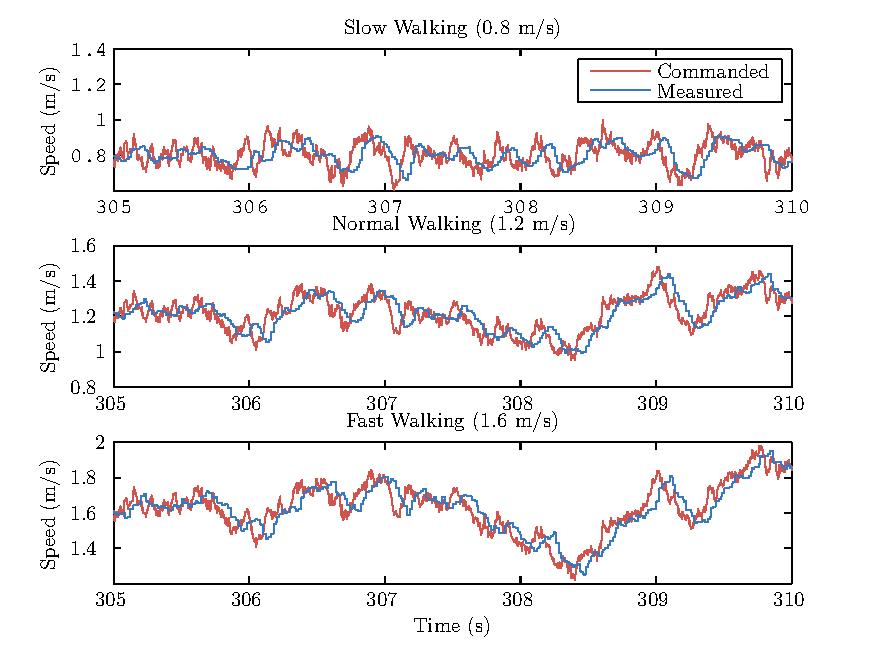
\includegraphics{figures/input_vs_output.pdf}
  \caption{Generated input signal (black) and actual treadmill belt movement
                (red) for average speeds of 0.8, 1.2, and 1.6 m/s, respectively}
  \label{fig:input_output}
\end{figure}

For further analysis, the input and output signals were transformed into the 
frequency domain through the Fast Fourier algorithm, and the results are
shown in Figure~\ref{fig:freq_analysis}.  It was observed that for the 1.2 $m \cdot s^{-1}$
average walking speed, the amplitude of the output is significantly lower 
than the amplitude of the input signal at lower frequencies.  Additionally, the 
amplitude of output signal in the 0.8 $m \cdot s^{-1}$ walking speed begins to attenuate 
around 2 Hz, which is a noticeably lower frequency than the other walking 
speeds.  

\begin{figure}
  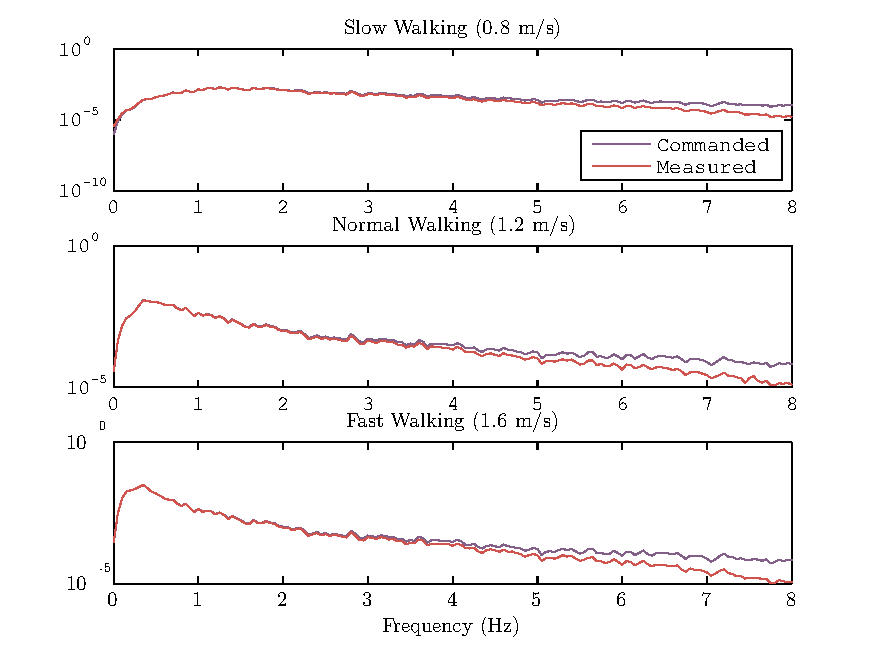
\includegraphics{figures/frequency_analysis.pdf}
  \caption{Frequency analysis of the  input (black) and output (red)
                for average speeds of 0.8, 1.2, and 1.6 m/s, respectively}
  \label{fig:freq_analysis}
\end{figure}

\section{Processed Data}

We developed a command line data processing tool for common gait computations
and provide the processed data from this. The tool was developed in Pythin and centered around two main
classes, one to store a complete trial in memory and a second to compute common
gait variables of interest.

The \verb|motek.DFlowData| class collects and stores all the raw data presented
in the previous section and applies several ``cleaning'' operations to put the
data into a usable form.

\begin{itemize}
  \item Loads the meta data file into a Python dictionary.
  \item Loads the DFlow mocap module TSV file into Pandas \verb|DataFrame|.
  \item Relabels the column headers to more meaningful names if this is
    specified in the meta data.
  \item Optionally identifies the missing values in the mocap marker data and
    replaces them with \verb|numpy.nan|.
  \item Optionally interpolates the missing marker values and replaces them
    with interpolated estimates using a variety of interpolation methods.
  \item Loads the D-Flow record moudle TSV file into a Pandas \verb|DataFrame|.
  \item Extracts the events and creates a dictionary mapping the event names in
    the meta data to the events detected in the record module file.
  \item Compensates the ground reaction loads for treadmill motion.
  \item Merges the data from the mocap module and record module into one data
    frame at the maximum common constant sample rate.
  \item Extracts sections of the data bounded by the events.
  \item Saves the cleaned data to disk.
\end{itemize}

The \verb|gait.WalkingData| class is then used to compute things such as gait
landmarks (toe off and heel strike times), basic 2D inverse dynamics, and to
store the data into a Pandas \verb|Panel| with each gait cycle on the main axis
at a specified sample rate. This data is also saved to disk in HDF5 format.

Figure~\ref{fig:angle-torque-comparison} compares the mean and standard
deviation of saggital plane joint angles and torques from the perturbed gait
cycles and the unperturbed gait cycles computed from trial 20 for 120 gait
cycles. The variation in the dynamics is larger for the perturbed gait cycles.

\begin{figure}
  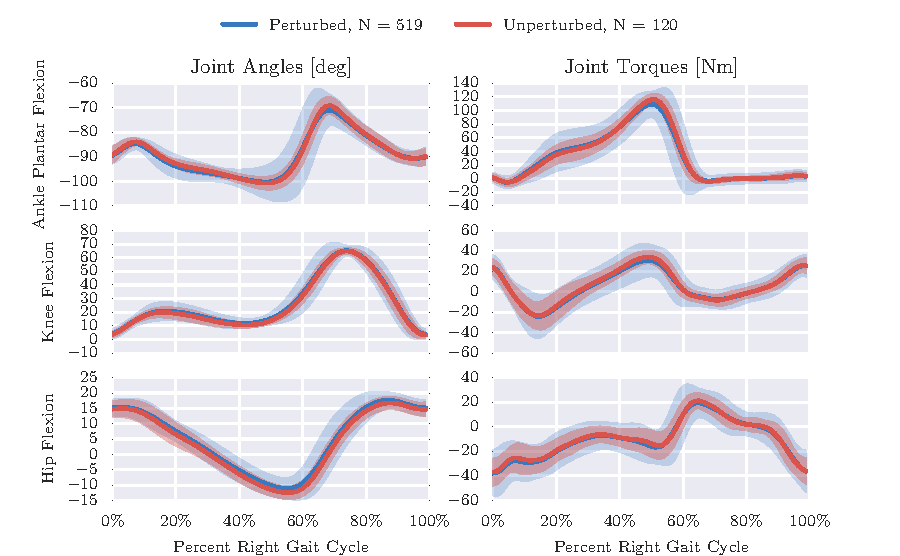
\includegraphics{figures/unperturbed-perturbed-comparison.pdf}
  \caption{Mean (solid, dashed) and $2\sigma$ (shaded) ($N=120$) joint angles
    and torques from both unperturbed (purple) and perturbed (blue) gait cycles
    from trial 20.}
  \label{fig:angle-torque-comparison}
\end{figure}

Figure~\ref{fig:gait-cycle-stats-comparison} compares the distribution in
several statistics of the unperturbed and perturbed gait cycles.

\begin{figure}
  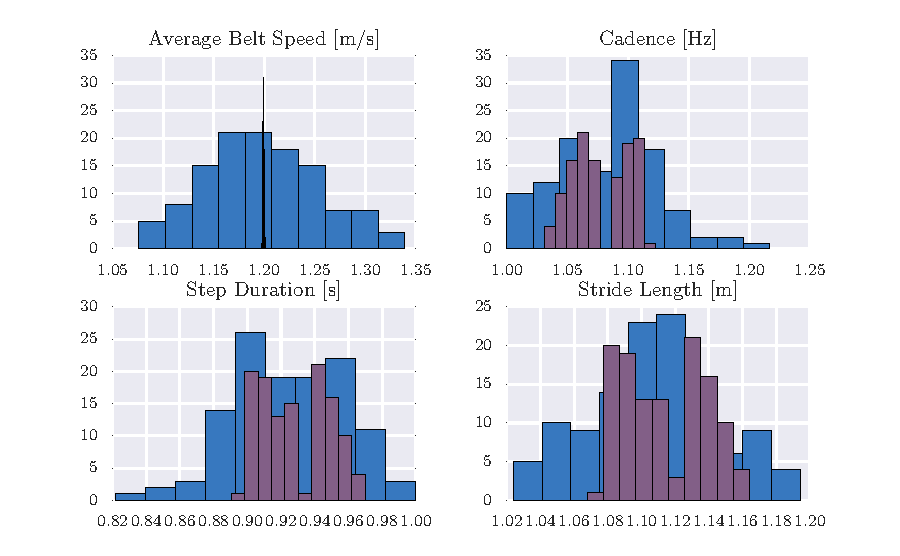
\includegraphics{figures/unperturbed-perturbed-hist-comparison.pdf}
  \caption{Histograms of the average belt speed, cadence, step duration, and
    stride length which compare 120 gait cycles for the unperturbed (purple)
    and perturbed (blue).}
  \label{fig:gait-cycle-stats-comparison}
\end{figure}

\section{Conclusion}

We have presented the details of what we believe to be a rich dataset of motion
and ground reaction loads humans exhibit when recovering from minor
longitudinal perturbations. The data provides a large sample of gait cycles
from both unperturbed and perturbed walking at three different nominal speeds.
The raw data is provided for reuse with sufficient detail with regards to meta
data and technical details. In addition to the data, we provide software that
can process the data for cleaning purposes and to produce typical saggital
plane gait variables of interest. Among other uses, we believe the dataset is
ideally suited for control identification purposes. Many researchers are
working on mathematical models for control in gait and this dataset provides
both a way to validate these models and data that can be used to generate
models.

\end{document}
